\documentclass{article}

% Official CS230 milestone setup. The final option displays the author block.
\PassOptionsToPackage{numbers,compress}{natbib}
\usepackage[final]{neurips_2026}
\usepackage[utf8]{inputenc}
\usepackage[T1]{fontenc}
\usepackage{hyperref}
\usepackage{url}
\usepackage{xurl}
\usepackage{booktabs}
\usepackage{amsmath}
\usepackage{amsfonts}
\usepackage{nicefrac}
\usepackage{microtype}
\usepackage{xcolor}
\usepackage{graphicx}
\newcommand{\pagelimit}{3}

\title{More Ball for Your Buck: Scouting Undervalued NBA Players}
\author{Elliott Ou \\
  \texttt{elliotto@stanford.edu}}

\begin{document}
\maketitle

\section{Introduction}
NBA teams must decide which players to sign, keep, or trade while managing their
salary costs. These decisions require teams to consider both a player's expected
performance and the cost of their contract. A player who improves while on an
inexpensive contract can help a team strengthen its roster, while an expensive
player whose performance declines can limit the team's options. Evaluating these
decisions requires looking beyond what a player produced last season and
considering what they are likely to contribute next season.

Previous work has studied NBA player performance relative to salary
\cite{lautier2023}. This project aims to predict next-season performance and use
those predictions to identify players who may provide good value at their salary.
It also examines expected improvements and declines, which could help teams
evaluate whether to acquire, retain, or trade a player.

Using historical NBA player data, this project applies neural networks to
predict next-season performance and playing time.

\section{Dataset}
The dataset contains 11,272 examples from NBA regular seasons between 1996--97 and
2025--26. Each example pairs a player's statistics from one season with their
performance in the following season. Statistics come from Sumitro Datta's
Basketball-Reference dataset \cite{datta2026}, and NBA PIE values come from
SportsDataverse \cite{sportsdataverse2026}. Salary data come from Bill Mill's
\texttt{nba\_data} archive \cite{mill2026}, Logan Lauton's NBA Player HUD
\cite{lauton2026}, Ram Vibhakar's basketball-analytics archive
\cite{vibhakar2026}, Erik Gregory Webb's NBA Salaries dataset \cite{webb2026},
and MrBridge's HoopsHype salary mirror \cite{mrbridge2026}. Salaries are available
for 11,176 examples. The 96 examples without salaries are retained for
performance training. Datta's Kaggle dataset is listed under CC0 (Public Domain).
Other sources, including NBA and Basketball-Reference data, have separate terms
of use.

Player names and IDs were used to match records across datasets. For traded
players, combined statistics from all their teams were used to keep one record
per season. Only regular-season statistics were included. An example requires
records in two consecutive seasons, so the models do not predict whether a
player will leave the NBA.

Examples were randomly split into 7,890 training (70\%), 1,691 development
(15\%), and 1,691 test examples (15\%), using seed 42. Seasons were not split by
date, and the same player can appear in different sets in different years. There
are 22 inputs: 17 numerical features covering age, playing time, basic statistics,
and advanced statistics, plus five one-hot position columns. Salary and player
identifiers are not model inputs.

Missing inputs are filled with training-set feature medians. Numerical inputs
are standardized separately for each season using that season's training mean
and standard deviation; those values are also applied to development and test
data. Missing outputs are not filled in. Two training examples lack WS/48 or BPM
values needed for targets or baselines, so these models and PCA use 7,888
examples; PIE and minutes use all 7,890. All development and test examples have
the required values. No pretrained models or data augmentation were used.

\section{Approach}
The proposal originally focused on predicting Player Impact Estimate (PIE).
The project now uses four separate neural networks, one each for PIE, Win Shares
per 48 minutes (WS/48), Box Plus/Minus (BPM), and total regular-season minutes.
The four predictions are combined into one score using principal component
analysis (PCA).

\paragraph{Neural networks.}
All four networks use the 22 inputs described in Section~2. They were implemented
in NumPy \cite{harris2020}, each with two ReLU hidden layers and one linear
output neuron. Weights use He initialization \cite{he2015}. Each network is
trained separately using mean squared error with L2 regularization:
\begin{equation}
  \mathcal{L}=\frac{1}{m}\sum_{i=1}^{m}
  \left(\widehat{y}_i-y_i\right)^2
  +\frac{\lambda}{2}\sum_{\ell}
  \left(\|W_{\ell}\|_F^2+\|b_{\ell}\|_2^2\right).
\end{equation}
Here, $y_i$ is the target and $\widehat{y}_i$ is the prediction.
PIE targets keep their original values; the other targets are standardized using
training-set means and standard deviations. Predictions are converted back
before evaluation and PCA, with negative minute predictions set to zero.
Training uses Adam \cite{kingma2015}, batch size 64, $\lambda=10^{-4}$, and at most
300 epochs. Training stops if development RMSE does not improve for 25 epochs,
and the weights from the best epoch are saved. All selected models use 10\%
dropout \cite{srivastava2014} during training. Dropout is turned off when
calculating reported errors.

Initial model selection compared hidden-layer widths, learning rates, and
dropout in 69 runs for PIE, WS/48, and BPM, plus six for minutes; each run used
seed 42. A five-seed comparison found that one-hidden-layer candidates had the
lowest mean individual-target RMSE. However, the seed-42 one-layer bundle had a
slightly higher development composite RMSE (0.7609) than the two-layer bundle
(0.7568), so we retain the two-layer models as primary.

A separate five-seed comparison of two-layer widths found the lowest mean
individual-target RMSE with widths 128--64 for PIE, 64--32 for WS/48, 32--16
for BPM, and 32--16 for minutes. Combining these target-specific candidates gave
mean development composite RMSE 0.7596 (SD 0.0019), compared with 0.7606
(SD 0.0029) for the existing widths. The difference is small, so the current
two-layer widths remain in the primary results pending stronger evidence.

\paragraph{PCA and baseline.}
PCA combines the four predicted statistics into one overall performance score.
Previous research has also used PCA for NBA player evaluation \cite{oliveira2024}.
Using scikit-learn \cite{pedregosa2011}, PCA is fitted on actual next-season
training values for PIE, WS/48, BPM, and total minutes. Each variable is
standardized using its training mean and standard deviation.

The first component uses weights approximately $w=(0.516,0.528,0.561,0.374)$.
It explains 72.36\% of the variation in the standardized training values; this
is not prediction accuracy. The score is scaled to training mean zero and
standard deviation one. The same fixed transformation is used for predicted
statistics, actual outcomes, and the baseline.

A baseline checks whether the neural networks improve on a simple prediction
rule. Here, the baseline assumes that each player will repeat their
previous-season statistics and total minutes. Reporting the networks' error
alone would not show whether their additional complexity provides a useful
improvement over this rule.

We compare the methods using RMSE and MAE, which is less affected by a few large
errors. Errors for individual outputs are reported in their original units;
composite errors use training-composite standard-deviation units. Each network
is trained on its own target, and the combined PCA score is evaluated afterward.

\paragraph{Remaining work.}
First, normalize listed salaries by the corresponding season's salary cap and
fit a training-only salary--performance benchmark, including rookie contracts.
Next, compare forecast-based value shortlists with prior-performance shortlists
on development data. Then evaluate simpler regressions, age/position/playing-time
subgroups, and any low-minute reliability policy without optimizing it on test
results. Finally, plan forward-in-time evaluation with a genuinely untouched
future assessment; the currently examined test split cannot provide a new
independent confirmation of a redesigned method.

\section{Partial Results}
Table~\ref{tab:dev} reports development results from the primary two-hidden-layer
models. All four targets improve on persistence RMSE. The minutes network reduces
RMSE from 677.54 to 589.94 minutes (12.93\%); the four-stat composite reduces it
from 0.9066 to 0.7568 (16.53\%). Adding minutes changes the composite's definition,
so a lower RMSE than a previous three-stat composite does not establish that the
new definition is a better basketball metric.

\begin{table}[ht]
  \centering
  \small
  \setlength{\tabcolsep}{4pt}
  \begin{tabular}{lccrr}
    \toprule
    Target & Hidden widths & Learning rate & Baseline RMSE & Model RMSE \\
    \midrule
    PIE & 32, 16 & 0.001 & 0.04584 & 0.03548 \\
    WS/48 & 128, 64 & 0.001 & 0.08279 & 0.07068 \\
    BPM & 32, 16 & 0.003 & 3.70394 & 3.13535 \\
    Total minutes & 64, 32 & 0.001 & 677.54 & 589.94 \\
    PCA composite & --- & --- & 0.90660 & 0.75676 \\
    \bottomrule
  \end{tabular}
  \caption{Development performance on 1,691 examples. Each target has different
  units, so error magnitudes should not be compared across rows.}
  \label{tab:dev}
\end{table}

The one-layer alternative's seed-42 development composite RMSE was 0.7609,
slightly higher than the primary two-layer model's 0.7568. The one-layer
candidate's favorable average individual-target rankings therefore did not
yield a lower composite error in that run.

The primary two-hidden-layer four-stat pipeline was evaluated on the original
test split (Table~\ref{tab:loss}); the one-layer and new width-search candidates
were not. That split had already been inspected during earlier three-stat
development, before the four-stat design was fixed. These are \emph{exploratory
follow-up test results}, not independent final confirmation. No weights or PCA
settings changed during that evaluation.

\begin{table}[ht]
  \centering
  \small
  \begin{tabular}{lrrr}
    \toprule
    Split & Composite MSE & Baseline MSE & Composite MAE \\
    \midrule
    Training & 0.5841 & 0.9560 & 0.4644 \\
    Development & 0.5727 & 0.8219 & 0.4878 \\
    Test (follow-up) & 1.1840 & 2.0520 & 0.4938 \\
    \bottomrule
  \end{tabular}
  \caption{Final composite loss with dropout disabled and all eligible rows
  retained: 7,888 training and 1,691 examples in each evaluation split.}
  \label{tab:loss}
\end{table}

For the primary two-layer pipeline, test composite RMSE is 1.0881 versus baseline
1.4325 (24.04\% reduction), but
extreme short appearances strongly affect squared error. A two-minute
Kuzminskas season with source-listed PIE $-4.0$ contributes 57.84\% of composite
test squared error. A prior one-minute season with BPM 242.2 for Mitrou-Long
also creates an extreme persistence error. These observations are retained,
rather than removed after inspecting test performance. Composite MAE changes
little between development and test (0.4878 versus 0.4938), unlike MSE
(Figure~\ref{fig:loss}). Thus, the MSE increase alone is insufficient evidence
of broad overfitting. Individual learning curves show declining training loss
after development loss plateaus, supporting early stopping; they do not establish
an irreducible-error level or prove absence of bias. No per-epoch test curve was
recorded. Plots use Matplotlib \cite{hunter2007}.

\begin{figure}[ht]
  \centering
  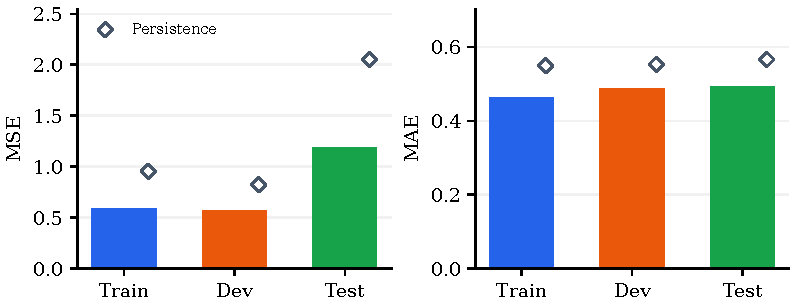
\includegraphics[width=\linewidth]{figures/composite_losses.pdf}
  \caption{Primary two-layer frozen-composite train/development/test error. Bars show model errors;
  diamonds show persistence. The test split is the previously examined follow-up
  split. Similar MAE and larger test MSE highlight sensitivity to extreme errors.}
  \label{fig:loss}
\end{figure}

\clearpage
\section*{References}
\renewcommand{\bibsection}{}
\medskip
{\small
\bibliographystyle{plainnat}
\bibliography{references}
}
\end{document}
